%%%%%%%%%%%%%%%%%%%%%%%%%%%%%%%%%%%%%%%%%%%%%%%%%%%
%% LaTeX book template                           %%
%% Author:  Amber Jain (http://amberj.devio.us/) %%
%% License: ISC license                          %%
%%%%%%%%%%%%%%%%%%%%%%%%%%%%%%%%%%%%%%%%%%%%%%%%%%%

\documentclass[a4paper,11pt]{book}
\usepackage[T1]{fontenc}
\usepackage[utf8]{inputenc}
\usepackage{lmodern}
\usepackage{hyperref}
\usepackage{graphicx}
\usepackage[english]{babel}

% title and subtitle
\title{\Huge \textbf{Unified Heteregeneous Networking Middleware Project Report}  \\ 
\huge \vspace{5mm} Fall 2015 }
% Author
\author{\textsc{Jincheng Li}}

\begin{document}

\frontmatter
\maketitle

% Auto-generated table of contents, list of figures and list of tables %
\tableofcontents
\mainmatter

% NEW CHAPTER! %
\chapter{Introduction}
Devices with Internet access today are becoming increasingly mobile. The Heterogeneous Networking Middleware project provides a mechanism for devices to seamlessly handle network mobility, and make intelligent decisions about how and when to use different networks across multiple interfaces. \\
The project started in 2012 in the IRT lab and underwent significant development from 2012 to 2013. After a period of inactivity, it was restarted in Spring 2015 and continued until now (Fall 2015). \\
The prototype for this project started with a demo on Linux and is currently shifting to Android. Some work was done last semester to port the Linux implementation to Android, while this semester we took a different approach and re-implemented some of the necessary functionalities within the Android Java Frameork. \\
In this report, I will cover existing work before I started contirbuting to the project, research on Android framework's networking stack, and what was done this semester to implement the middleware in Android.

\chapter{Existing Work}
Prior to me being involved in the project, a lot of work has been done on the research on heterogeneous networks and Linux prototype implementation. Porting to Android only started in Spring 2015. 

\section{Protocols}
\subsection{HIP}
\subsection{MIP}
\subsection{MIH}

\section{Linux Demo Architecture}

\chapter{Android Networking Stack}
In order to understand how Android performs network switching and the functionalities it provides similar to MIH, a fair amount of time was spent this semester researching the architecture of Android's networking stack. Here we present the details of our findings.

\section{Android Architecture}
Before we talk about the Android networking stack, we first introduce the architecture of the Android platform. Broadly speaking, Android consists of five layers: Linux kernel, HAL, Android runtime + native libraries, Android Framework, and user applications. These five layers are laid out in the following diagram: % elaborate...

% android architecture diagram here
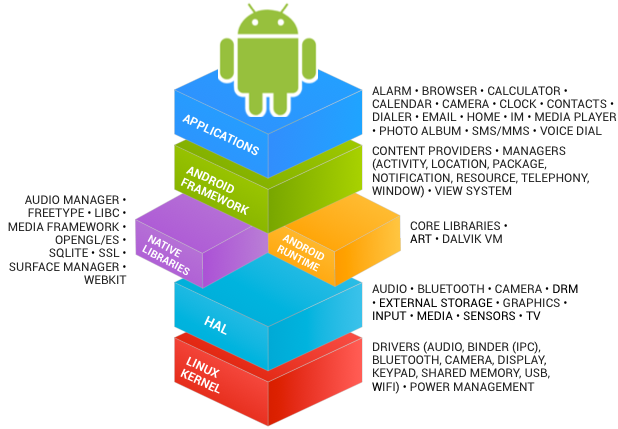
\includegraphics[width=\textwidth]{figures/android_framework_details.png}

At the bottom of the Android software stack is the Linux kernel, which provides a level of abstraction between the device hardware and the upper layers of Android. The kernel provides typical low-level system services such as process, memory management, and also includes essential device drivers for hardware such as cellular and WiFi NICs. \\
The hardware abstraction layer (HAL) defines a standard interface for hardware vendors to implement and allows Android to be agnostic about lower-level driver implementations. We don't discuss HAL at any more length here as it is not vital for our purposes. \\
Next comes the Android runtime (i.e. Davlik VM) and native libraries, which are implemented in C/C++. \\
Layered on top of the runtime and libraries is the Android Framework. This framework is implemented entirely in Java, and provides applications with an API that can be used to interact with system services, including UI, telephony, location, etc. This part of Android is what most of the research effort on Android this semester focused on. The final demo also directly modifies Android Framework's source code to integrate our middleware functionalities into the system. \\
Finally on the top level is user applications that interact directly with the user. 

\section{General Networking}
The following classes deal with network connectivity for all types of networks (cellular, WiFi, or ethernet). This is done through an abstraction called NetworkAgent that encapsulates different types of networks into a common interface, as is explained in more detail later in this section.

\subsection{ConnectivityManager}
In general, classes with a ``Manager'' suffix are singleton classes exposed as part of the Android API for applications. They serve as the interface between application developers and the Android framework. Methods in these classes do not usually contain intricate program logic, but simply call some other system service class (e.g. methods in ConnectivityManager call corresponding methods in ConnectivtyService) which actually implements the required functionality. \\
In the case of ConnectivityManager, it is reponsible for answering queries about the state of network connectivity, and for notifying applications about network connectivity changes. Additionally, it allows applications to request or select certain networks for their data traffic. This last feature is most relevant to our research. The method involved here is \verb|requestNetwork|, which takes as its input a \verb|NetworkRequest|, and a \verb|NetworkCallback|. 

\subsection{ConnectivityService}

\subsection{NetworkAgent and NetworkAgentInfo}

\section{WiFi Networks}

\subsection{WifiManager}
The WifiManager class is exposed as part of Android's application API. It provides methods for applications to manage all aspects of WiFi connectivity.

\subsection{WifiService}

\subsection{WifiStateMachine}

\subsection{WifiAutoJoinController}

\section{Cellular Networks}
\subsection{TelephonyManager}
\subsection{DataConnection}

\section{Another section heading}
Lorem ipsum dolor sit amet, consectetur adipisicing elit, sed do eiusmod tempor incididunt ut labore et dolore magna aliqua. Ut enim ad minim veniam, quis nostrud exercitation ullamco laboris nisi ut aliquip ex ea commodo consequat.

% Sample table                                        %
% Source: www1.maths.leeds.ac.uk/latex/TableHelp1.pdf %
\begin{table}[ht]
\caption{Sample table} % title of Table
\centering % used for centering table
\begin{tabular}{c c c c}
% centered columns (4 columns)
\hline\hline %inserts double horizontal lines
S. No. & Column\#1 & Column\#2 & Column\#3 \\ [0.5ex]
% inserts table
% heading
\hline % inserts single horizontal line
1 & 50 & 837 & 970 \\
2 & 47 & 877 & 230 \\
3 & 31 & 25 & 415 \\
4 & 35 & 144 & 2356 \\
5 & 45 & 300 & 556 \\ [1ex] % [1ex] adds vertical space
\hline %inserts single line
\end{tabular}
\label{table:nonlin} % is used to refer this table in the text
\end{table}

\chapter{Implementation in Android}

\section{Working with the Android Framework}
This section describes the necessary steps to set up and work with the Android framework. Most of this information can also be found on the AOSP (Android open-source project) site online. This guide simply documents the specific steps involved in this project. \\

\section{Final Demo}

\end{document}
